\section{Forsøg med Hooks lov}
I anledning af vigtigheden af Hookes lov for denne opgave har jeg opstillet nogle forsøg. Forsøgene har dels til formål at eftervise validiteten af Hookes lov samt at anskueliggøre ideen om at kovalente bindinger kan betragtes som fjedre. Der er i alt 4 forsøg: Det første skal vise at den kraft som en fjeder trækker med, når den bliver trukket i er direkte proportionelt med afstanden som fjederen bliver trukket ud samt at proportionalitetsfaktoren er fjederkonstanten k. Det andet forsøg skal vise at stedfunktionen for et objekt der laver en oscillerende bevægelse kan skrives på formen $x(t) = A \cdot sin(B t + C) + D$, hvor A, B, C er konstanter. A bestemmes som amplituden på udslagene og B bestemmes som $B=\sqrt[2]{\frac{k}{m}}$. Det tredje forsøg skal vise, at hvis vi har et system af to fjedre, som er helt ens, og vi hænger en masse i de to fjedre, vil fjederkonstanten for systemet blive lig summen af de to fjedres fjederkonstanter. Det fjerde forsøg skal vise, at hvis vi har et system med flere forskellige fjedre og betragter dem som \textbf{én} samlet fjeder, vil fjederkonstanten for systemet af fjedre være lig summen af de fjederkonstanter for fjedrene, som er med i systemet. Det fjerde forsøg er en udvidelse af det tredje forsøg. 

\subsection{Forsøg 1}
En luftpudebænk blev sat op og 2 kroge blev monteret. Én for enden af luftpudebænken og én på en vogn. Der blev fastgjort en fjeder mellem de to kroge. Derefter blev der trukket i vognen og målt sammenhørende værdier mellem afstanden som vognen blev trukket ud og kraften målt på et newtonmeter, som blev brugt til at hive i vognen med. Efter indtastning af data i programmet LoggerPro blev følgende graf tegnet ved at prøve at passe en proportionel regression ned over den målte data. 

\begin{center}
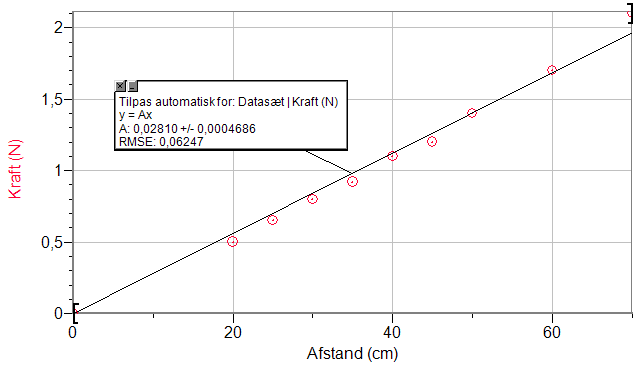
\includegraphics[scale=0.7]{Billeder/graf1}
\end{center}

Vi kan konkludere ud fra $Root-mean-square$-værdien, der er på 0.06247, at en proportionel regression passer godt på den målte data. Altså må Hookes lov $F=k \cdot x$ gælde (\textbf{Notér} at fortegnet her bliver ignoreret, da vi ikke regner med retninger). Ydermere kan vi sige at fjederkonstanten for den pågældende fjeder har en værdi på $k=0.0281\frac{N}{cm} = 2.81 \frac{N}{m}$ da dette er hældningskoefficienten på vores lineære regression og altså k i $F=k \cdot x$
\\

Den data, der ligger til grunde for forsøget og selve forsøgsopsætningen kan ses på bilag 1. 
\\

\subsection{Forsøg 2}
I dette forsøg blev en fjeder, \emph{ikke} den samme som i forsøg 1, monteret til et stativ og et lod blev hængt i fjederen. Med en Go!Motion ultralydssensor blev afstanden til loddet målt til sammenhørende tidspunkter. Ultralydssensoren var sat til en computer og sendte automatisk data ind i programmet LoggerPro, der behandlede dataen og plottede den. Der blev foretaget en regression på datapunkterne på formen $x = A \cdot (B \cdot t + C) + D$. Dette kan ses på følgende billede: 
\begin{center}
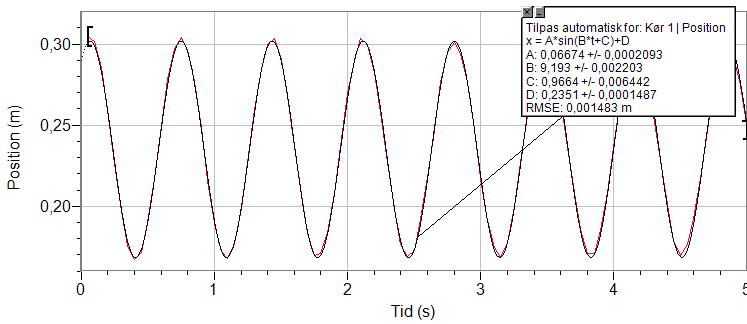
\includegraphics[scale=0.7]{Billeder/graf2}
\end{center}

Som det fremgår af $root-mean-square$-værdien af den regression der er lavet over dataen passer den definerede funktion. Det var dette vi gerne ville vise. Herved har vi vist at en oscillerende bevægelse kan skrives på formen: $x = A \cdot (B \cdot t + C) + D$, hvor $B=\sqrt[2]{\dfrac{k}{m}}$. Vi definerer nogle gange $\omega = \sqrt[2]{\dfrac{k}{m}}$ så forskriften kommer til at blive $x(t) = A \cdot (\omega t + C) + D$.
\\

Dataen der er brugt til at lave regressionen og forsøgsopsætningen kan ses på bilag 2.
\subsection{Forsøg 3}
I dette forsøg blev 2 fjedre, identiske til den som blev brugt i forsøg 1, hængt op på et stativ og et lod blev sat til dem og loddet blev sat i bevægelse. En Go!Motion ultralydssensor målte afstanden til loddet til en tid og plottede det i programmet LoggerPro. Plottet så sådan ud:

\begin{center}
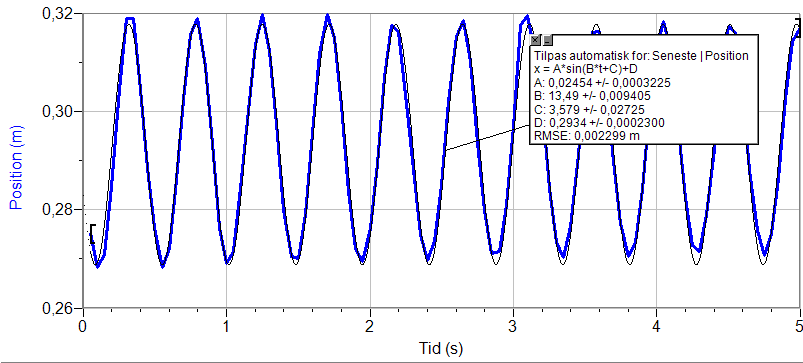
\includegraphics[scale=0.7]{Billeder/graf3}
\end{center}

Her kan vi se, at værdien for B eller $B = \omega = \sqrt[2]{\dfrac{k}{m}}=13.49$. Men da vi kender massen af loddet som blev brugt som $m=32.45g$, (\emph{denne værdi blev målt inden forsøget}), kan vi beregne fjederkonstanten af dette system som:
$k=\omega^2 \cdot m = \frac{13.49}{s} \cdot 32.45g = 5.879 \frac{N}{m}$. Men da vi fandt ud af at fjederkonstanten for forsøg 1 var $k=2.81\frac{N}{m}$ skulle den forventede fjederkonstant for dette forsøg være $2 \cdot 2.81 \frac{N}{m}= 5.62 \frac{N}{m}$. Det målte viste sig at være $5.879 \frac{N}{m}$, hvilket er meget tæt på den forventede værdi. Vi konkluderer at et system bestående af 2 af de samme fjedre får en fjederkonstant, der er lig summen af de 2 fjedre der er med i systemet. 

\subsection{Forsøg 4}
Dette forsøg skulle undersøge fjederkonstanten for en dobbeltbinding, som består af en $\pi-binding$ og en enkelt $\sigma-binding$. I forsøget blev der derfor brugt 3 fjedre, hvor 2 af fjedrene var ens. (2 de ens fjedre skulle symbolisere $\pi$-bindingen der er at finde på begge sider af sigmabindingen). Fjedrene blev hængt op på et stativ og en lodbåd med en vægt i blev hængt i fjedrene. De enkelte fjederkonstanter for fjedrene var hhv. $k_1 = 2.74\frac{N}{m}$ og $k_2=17.03 \frac{N}{m}$. Der var 2 fjedre med fjederkonstanten $k_1$ og én med fjederkonstanten $k_2$. Den forventede fjederkonstant for systemet var da $k_{system}= 2 \cdot k_1 + k_2$. Lodbåden med vægten i blev sat i bevægelse og en Go!Motion ultralydssensor sendte data til computeren, der i programmet LoggerPro behandlede dataen og plottede følgende efter at have givet LoggerPro en regression for harmonisk oscillerende bevægelse:

\begin{center}
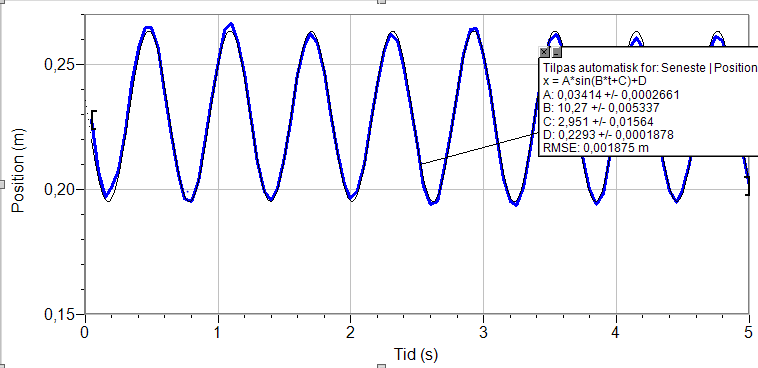
\includegraphics[scale=0.7]{Billeder/graf4}
\end{center}

$root-mean-square$-værdien er lav og regressionen passer derfor på dataen. Dette betyder at vi kan beregne fjederkonstanten, k, ud fra B værdien af den givne forskrift.
\\

Da $B=\sqrt[2]{\dfrac{k}{m}}$ og massen af det lod som blev brugt var 220g kan fjederkonstanten, k, løses i ovenstående ligning:
\\

$k=B^2 \cdot m = (10.27)^2 \cdot 220g = 23.2 \frac{N}{m}$
\\

Vores gæt på fjederkonstanten for dette system var: $2 \cdot k_1 + k_2 = 2 \cdot 2.74 \frac{N}{m} + 17.03 \frac{N}{m} = 22.51 \frac{N}{m}$. 

Disse to værdier er tæt nok på hinanden til at kunne sige, at der er en sammenhæng. Det må altså gælde at fjederkonstanten for et system med tre fjedre er lig summen af fjederkonstanterne for fjedrene der indgår i systemet. 
\\

\subsection{Delkonklusion}\label{sec:del}
Den målte data og den efterfølgende behandling af det selv samme, har eftervist Hookes lov om fjedre. Derudover har det også vist sig at et objekt med en masse, der hænger i fjeder og som sættes i bevægelse foretager en harmonisk oscillerende bevægelse, hvor fjederkonstanten kan bestemmes ud fra forskriften. Ydermere er der vist, at et system bestående af forskellige fjedre vil have en samlet fjederkonstant for systemet, som er lig summen af de individuelle fjederkonstanter.
\\

Vi vil nu på hvordan disse resultater relatere sig til kemien bag IR-spektroskopi.